\nocite{1030194}
\nocite{1369494}
\nocite{7969976}

\chapter{Thesis Background}
\label{sec:backgroundthesis}

This chapter is about the background of the thesis, in order to understand better further chapters and as a help and reference to reproduce the results of this thesis in the future. 

\section{PYNQ-Z2 Development Board}
\label{sec:pynq}
The \textit{PYNQ-Z2} is a development board designed for the Xilinx University Program. It is equipped with a Xilinx ZYNQ 7020 SoC (XC7Z020-1CLG400C), 512 MB of DDR3 RAM and 16 MB of QSPI Flash Storage. The board provides a clock reference thanks to a crystal oscillator with a frequency of 50 MHz. The reference clock is used by the PS and can be provided to the PL too. 

\begin{figure}[H]
\centering
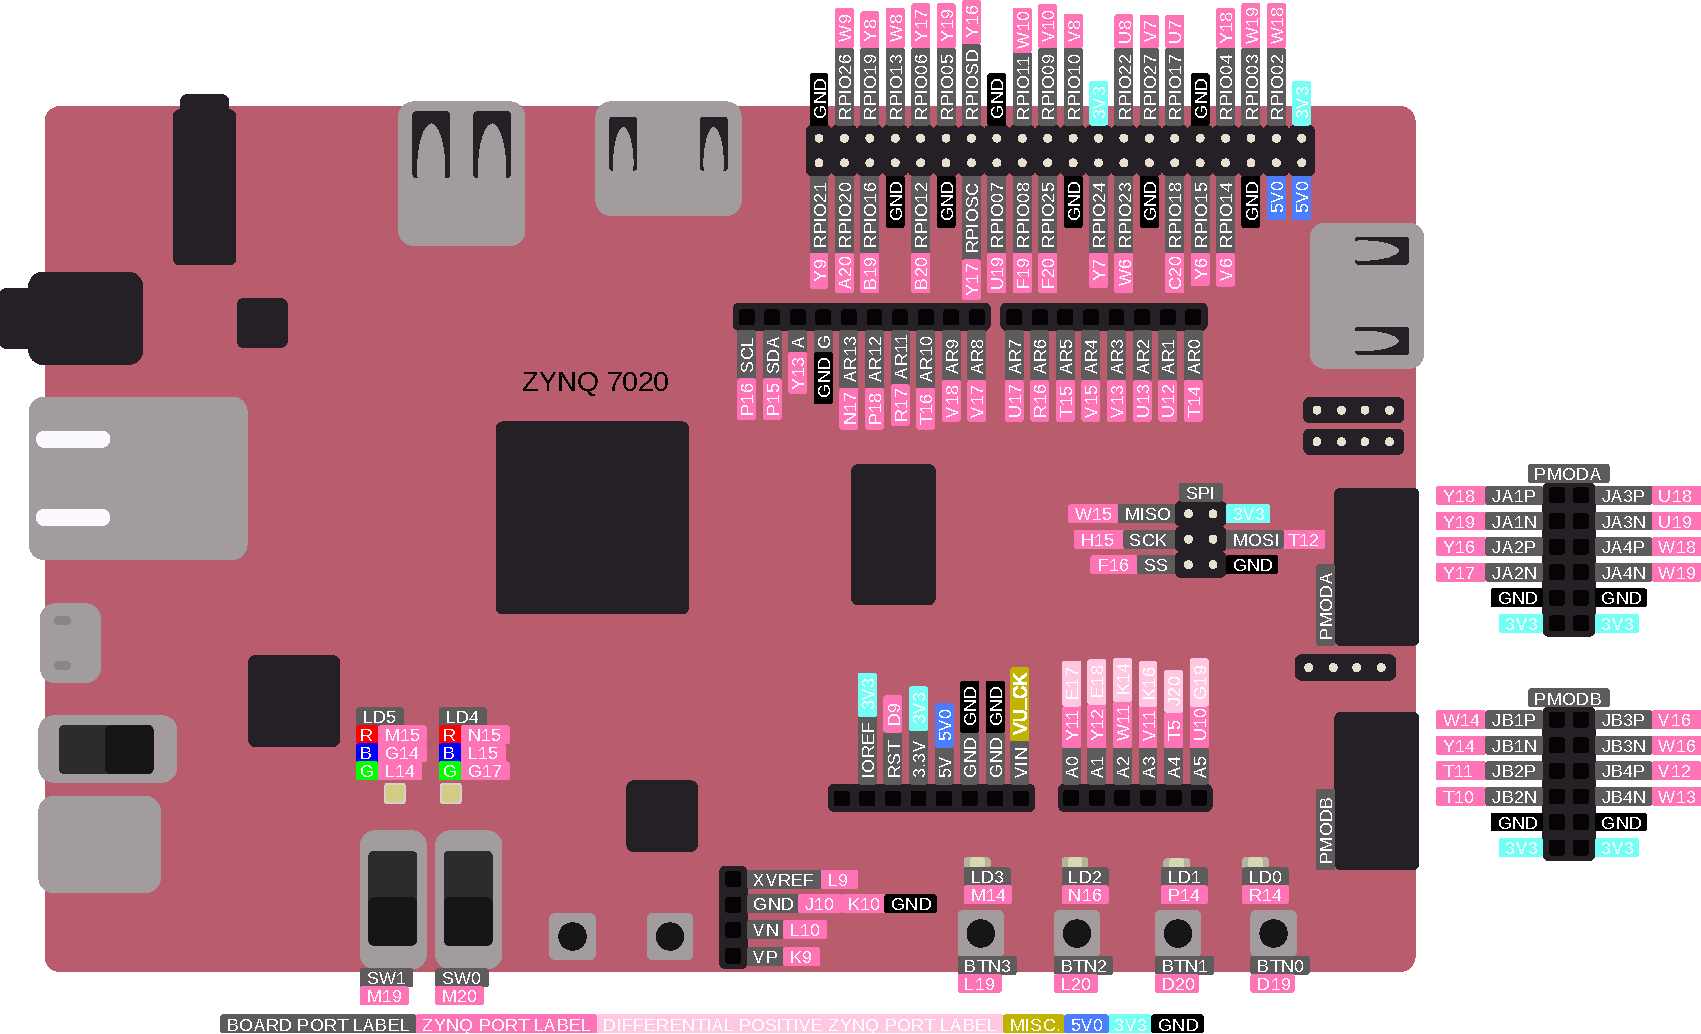
\includegraphics[width=0.7\linewidth]{images/chapter3/PINOUT.pdf}
\caption{Schematic of the PYNQ-Z2 Development Board}
\label{fig:pynqz2}
\end{figure}

The SoC is made of two subparts: a Processing System (PS) and a Programmable Logic (PL). The PS is the main part of the SoC, containing two 650 MHz ARM Cortex-A9 processors, 512 KB L2 Cache, 256 KB On-Chip Memory and other modules like FPUs, Flash Controller, DRAM Controller, GPIOs and so on.

\begin{figure}[H]
\centering
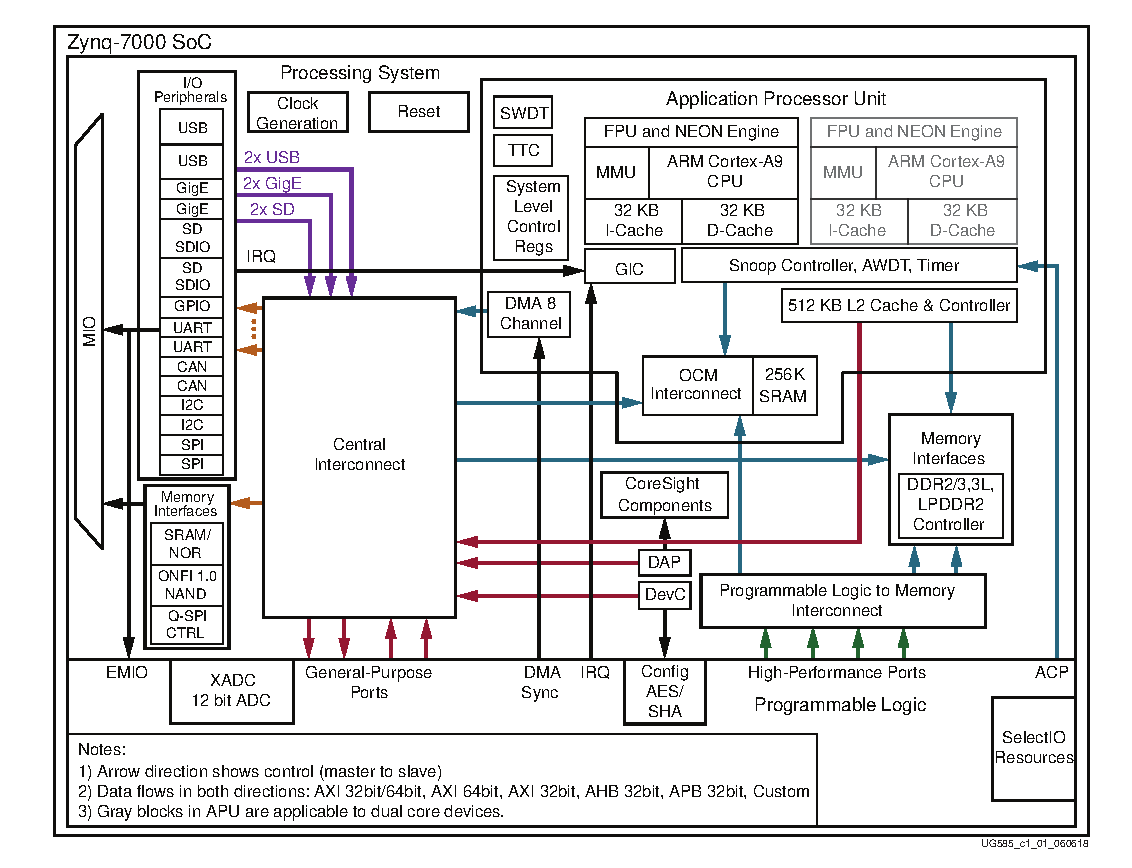
\includegraphics[width=1.0\linewidth]{images/chapter3/zynq.pdf}
\caption{Schematic of ZYNQ 7020 SoC}
\label{fig:zynq7020}
\end{figure}

A schematic is shown in Figure \ref{fig:zynq7020}. The second part is the PL, which consists in an FPGA with the following characteristics:

\begin{itemize}
    \item 13,300 logic slices, each with four 6-input LUTs and 8 flipflops
    \item 630 KB block RAM (BRAM)
    \item 220 DSP slices
    \item On-chip Xilinx analog-to-digital converter (XADC)
\end{itemize}

The PL can access the Processing System's memory space, as shown in Table \ref{tab:zynq_memory_map}, through High Performance and/or General Purpose AXI Ports. This enables the usage, for example, of the DDR3 RAM and the On-Chip Memory (OCM) from the PL. The board can be programmed through a JTAG interface, which allows uploading firmware to be executed from the PS or to program the PL via a bitstream. Moreover, it provides a virtual UART interface that can be used as input/output both for the PS and the PL.\bigskip

\begin{table}[ht]
\centering
\begin{tabular}{ |p{3cm}||p{3cm}||p{5cm}|  }
    \hline
    \multicolumn{3}{|c|}{Memory Mapping} \\
    \hline
    Address Start&Address End&Device \\
    \hline
    \texttt{0x00000000}&\texttt{0x3FFFFFFF}&DDR \& OCM\\
    \texttt{0x40000000}&\texttt{0xBFFFFFFF}&PL  \\
    \texttt{0xC0000000}&\texttt{0xDFFFFFFF}&Reserved\\
    \texttt{0xE0000000}&\texttt{0xE02FFFFF}&Memory mapped devices\\
    \texttt{0xE0300000}&\texttt{0xE0FFFFFF}&Reserved\\
    \texttt{0xE1000000}&\texttt{0xE3FFFFFF}&NAND, NOR\\
    \texttt{0xE4000000}&\texttt{0xE5FFFFFF}&SRAM\\
    \texttt{0xE6000000}&\texttt{0xF7FFFFFF}&Reserved\\
    \texttt{0xF8000000}&\texttt{0xF8FFFFFF}&AMBA APB Peripherals\\
    \texttt{0xF9000000}&\texttt{0xFBFFFFFF}&Reserved\\
    \texttt{0xFC000000}&\texttt{0xFDFFFFFF}&Linear QSPI - XIP\\
    \texttt{0xFE000000}&\texttt{0xFFEFFFFF}&Reserved\\
    \texttt{0xFFF00000}&\texttt{0xFFFFFFFF}&OCM \\
    \hline
\end{tabular}
\caption{ZYNQ 7020 SoC Memory Map}
\label{tab:zynq_memory_map}
\end{table}

% \begin{bytefield}{24}
%     \memsection{0xffff\_ffff}{0xfff0\_0000}{3}{PL}\\
%     \memsection{0xffef\_ffff}{0xfe00\_0000}{3}{PL}\\
%     \memsection{0xfdff\_ffff}{0xfc00\_0000}{3}{PL}\\
%     \memsection{0xfbff\_ffff}{0xf900\_0000}{3}{PL}\\
%     \memsection{0xf8ff\_ffff}{0xf800\_0000}{3}{PL}\\
%     \memsection{0xf7ff\_ffff}{0xe600\_0000}{3}{PL}\\
%     \memsection{0xe5ff\_ffff}{0xe400\_0000}{3}{PL}\\
%     \memsection{0xe3ff\_ffff}{0xe100\_0000}{3}{PL}\\
%     \memsection{0xe0ff\_ffff}{0xe030\_0000}{3}{PL}\\
%     \memsection{0xe02f\_ffff}{0xe000\_0000}{3}{PL}\\
%     \memsection{0xdfff\_ffff}{0xc000\_0000}{3}{PL}\\
%     \memsection{0xbfff\_ffff}{0x4000\_0000}{3}{PL}\\
%     \memsection{0x3fff\_ffff}{0x0000\_0000}{3}{OCM/DDR}
% \end{bytefield}


%%%%%%%%%%%%%%%%%%%%%%%%%%%%%%%%%%%%%%%%%%%%%%%%%%%%%%%%%%%%%%%%%%%%%%%%%
%%%%%%%%%%%%%%%%%%%%%%%%%%%%%%%%%%%%%%%%%%%%%%%%%%%%%%%%%%%%%%%%%%%%%%%%%
%%%%%%%%%%%%%%%%%%%%%%%%%%%%%%%%%%%%%%%%%%%%%%%%%%%%%%%%%%%%%%%%%%%%%%%%%
%%%%%%%%%%%%%%%%%%%%%%%%%%%%%%%%%%%%%%%%%%%%%%%%%%%%%%%%%%%%%%%%%%%%%%%%%
%%%%%%%%%%%%%%%%%%%%%%%%%%%%%%%%%%%%%%%%%%%%%%%%%%%%%%%%%%%%%%%%%%%%%%%%%
%%%%%%%%%%%%%%%%%%%%%%%%%%%%%%%%%%%%%%%%%%%%%%%%%%%%%%%%%%%%%%%%%%%%%%%%%
%%%%%%%%%%%%%%%%%%%%%%%%%%%%%%%%%%%%%%%%%%%%%%%%%%%%%%%%%%%%%%%%%%%%%%%%%
%%%%%%%%%%%%%%%%%%%%%%%%%%%%%%%%%%%%%%%%%%%%%%%%%%%%%%%%%%%%%%%%%%%%%%%%%
%%%%%%%%%%%%%%%%%%%%%%%%%%%%%%%%%%%%%%%%%%%%%%%%%%%%%%%%%%%%%%%%%%%%%%%%%
%%%%%%%%%%%%%%%%%%%%%%%%%%%%%%%%%%%%%%%%%%%%%%%%%%%%%%%%%%%%%%%%%%%%%%%%%
%%%%%%%%%%%%%%%%%%%%%%%%%%%%%%%%%%%%%%%%%%%%%%%%%%%%%%%%%%%%%%%%%%%%%%%%%
% \subsection{Configuration Ports}
%%%%%%%%%%%%%%%%%%%%%%%%%%%%%%%%%%%%%%%%%%%%%%%%%%%%%%%%%%%%%%%%%%%%%%%%%
%%%%%%%%%%%%%%%%%%%%%%%%%%%%%%%%%%%%%%%%%%%%%%%%%%%%%%%%%%%%%%%%%%%%%%%%%
%%%%%%%%%%%%%%%%%%%%%%%%%%%%%%%%%%%%%%%%%%%%%%%%%%%%%%%%%%%%%%%%%%%%%%%%%
%%%%%%%%%%%%%%%%%%%%%%%%%%%%%%%%%%%%%%%%%%%%%%%%%%%%%%%%%%%%%%%%%%%%%%%%%
%%%%%%%%%%%%%%%%%%%%%%%%%%%%%%%%%%%%%%%%%%%%%%%%%%%%%%%%%%%%%%%%%%%%%%%%%
%%%%%%%%%%%%%%%%%%%%%%%%%%%%%%%%%%%%%%%%%%%%%%%%%%%%%%%%%%%%%%%%%%%%%%%%%
%%%%%%%%%%%%%%%%%%%%%%%%%%%%%%%%%%%%%%%%%%%%%%%%%%%%%%%%%%%%%%%%%%%%%%%%%
%%%%%%%%%%%%%%%%%%%%%%%%%%%%%%%%%%%%%%%%%%%%%%%%%%%%%%%%%%%%%%%%%%%%%%%%%
%%%%%%%%%%%%%%%%%%%%%%%%%%%%%%%%%%%%%%%%%%%%%%%%%%%%%%%%%%%%%%%%%%%%%%%%%
%%%%%%%%%%%%%%%%%%%%%%%%%%%%%%%%%%%%%%%%%%%%%%%%%%%%%%%%%%%%%%%%%%%%%%%%%
%%%%%%%%%%%%%%%%%%%%%%%%%%%%%%%%%%%%%%%%%%%%%%%%%%%%%%%%%%%%%%%%%%%%%%%%%

\section{Xilinx soft-core: the MicroBlaze}

The Microblaze is a soft-core (or soft-microprocessor) designed for Xilinx's FPGAs. Introduced in 2002, it is based on a RISC architecture, with an ISA (Instruction Set Architecture) similar to the DLX architecture. It is a pipelined processor and, with few exceptions, the MicroBlaze can issue a new instruction every cycle, maintaining single-cycle throughput under most circumstances.\bigskip

The Microblaze has an interface to the AXI Interconnect, used to connect to other peripherals and memories. It has a dedicated bus, LMB Bus, for access to local-memory (FPGA's BRAMs): this can be used both for Instruction (ILMB) and Data (DLMB) storage.

\begin{figure}[H]
\centering
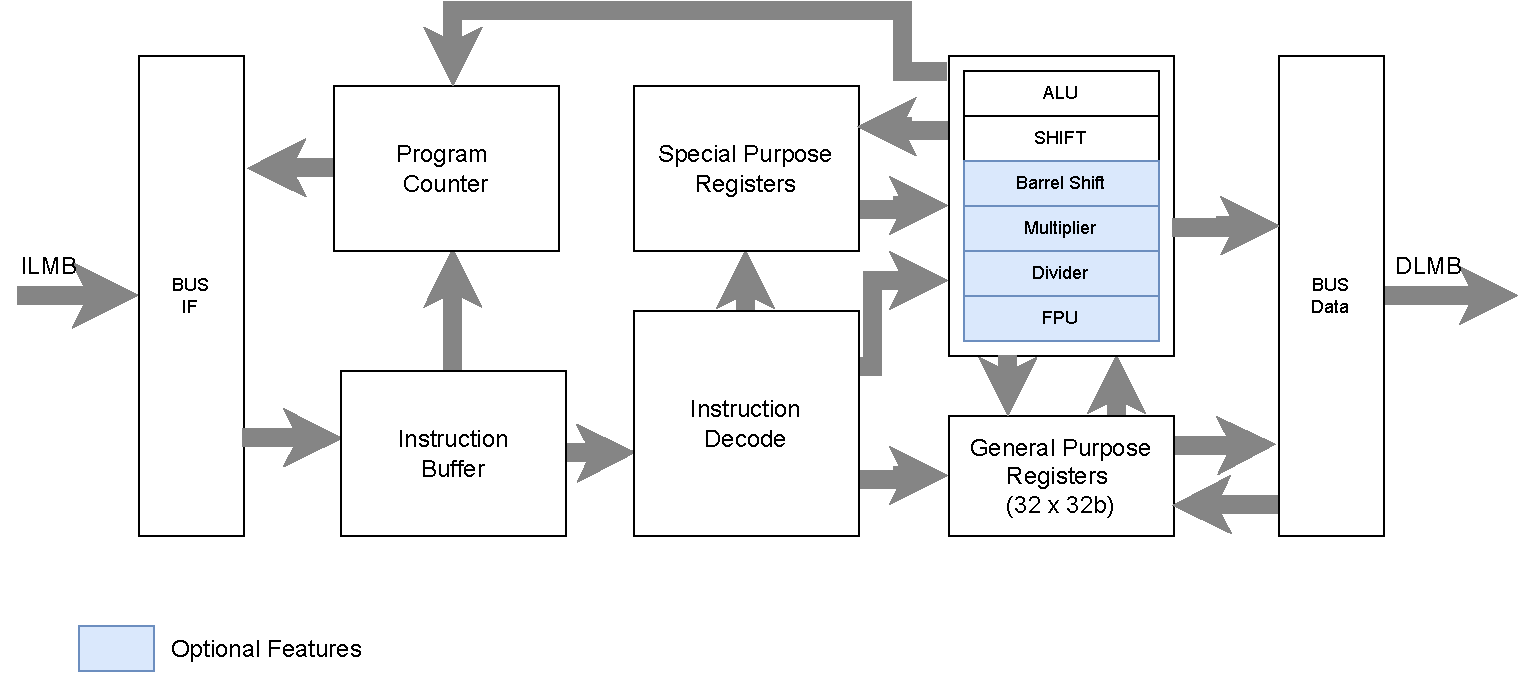
\includegraphics[width=0.8\linewidth]{images/chapter3/ublaze_arch.pdf}
\caption{\cite{anemaet2003microprocessor}Overview of a Microblaze SoftCore}
\label{fig:ublaze}
\end{figure}

A general overview of the Microblaze architecture is shown in Figure \ref{fig:ublaze}. Because it is meant for FPGAs, and FPGAs are flexible by construction, a Microblaze instance can be personalized in many ways to fit the user's needs. Examples of configurations are the cache size (or the cache can be enabled or disabled at all), pipeline depth (3-stage, 5-stage, or 8-stage) and bus interfaces. There are some presets, like the area-optimized one which uses a 3-stage pipeline and sacrifices clock frequency for the reduced logic area. The performance-optimized preset expands the execution pipeline to 5 stages. One of the most important configuration is related to the supported ISA: key processor instructions which are rarely used but more expensive to implement in hardware can be selectively added/removed (e.g. multiply, divide, and floating-point operations).

\section{Xilinx FPGA Standard Design Flow}

Xilinx offers a software suite for Xilinx's FPGAs. The provided software suite is \textit{Vivado Design Suite}, and this thesis has been developed using version 2021.1. The suite supports designers in all the steps of the design process, from the initial HDL design to the final FPGA bitstream generation. At each stage of the design flow, the design can perform analysis and verification, by performing logical simulations of the design, estimation of power consumption, constraints definition, I/O and clock planning, design rule checks (DRC) and modification of implementation results.\bigskip

Together with the HDL description, Vivado offers an IP catalog. IP stands for Intellectual Property, and each IP is an already developed and tested design ready to be integrated into the user's own design. An example of IP offered by default is the Microblaze IP, which contains the Microblaze core. The Vivado's Catalog is a comprehensive list of all the IP offered by different repositories: Xilinx's IP, IP obtained from third parties, and end-user designs targeted for reuse as IP in a single environment. \bigskip

One of the key features of the Vivado Design Suite is the choice given to the user to perform the design flow through the Graphical User Interface (GUI) or by TCL commands. The GUI, known as \textit{Vivado Integrated Design Environment} (IDE), allows the user to follow the evolution of the design visually from the HDL and IP instantiation up to its implementation on physical resources. The TCL commands allow the user to control the design flow by employing scripts. The interesting thing is that each action performed by the user in the GUI corresponds to an exact TCL command that can be seen from the TCL Console available in the IDE. This allows the user to understand what is the TCL command for that specific action and to script the design flow easily. 

\subsection{Steps towards the Bitstream Generation}
\label{sec:bitstreamgen}

The starting point of the design flow is the description of the system. The description can be made of a set of HDL files (Vivado supports Verilog, VHDL and SystemVerilog), a set of design constraints (XDXC) and a set of IP instantiations. \bigskip 

Thus, a design can be a combination of IPs and hand-written HDL code or it can be a full IP-centric design, where the user instantiates IPs he/she wants to use and interconnects them (usually via AXI Interface but also other interfaces or custom interfaces, it depends on the IP). For the IP-centric design flow, Vivado offers the \textit{Block Design} tool, which allows the user to visually instantiate e move and connect IPs visually, where each IP corresponds to a block, and to connect them by drawing connections similar to a schematic or using connection automation features provided with a set of DRCs (to ensure proper IP configuration and connectivity), as shown in Figure \ref{fig:block_design_example}. \bigskip

% include image
\begin{figure}[H]
\centering
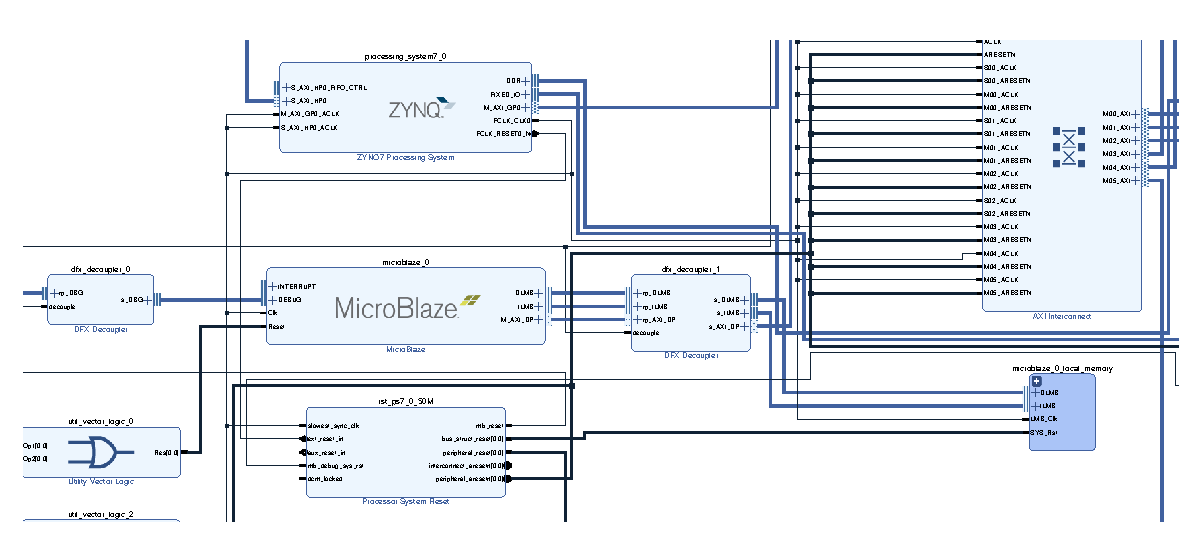
\includegraphics[width=0.75\linewidth]{images/chapter3/design_example-cropped.pdf}
\caption{Example of Block Design}
\label{fig:block_design_example}
\end{figure}

Moreover, the Block Design Tool allows the user to define the memory mapping of the AXI peripherals concerning the AXI masters. In the example above there are two masters, the ZYNQ7 Processing System and a Microblaze, and both of them are connected to the same AXI Interconnect IP. All the other peripherals are connected to the same AXI Interconnect IP. So, in the end, there are two separated memory address spaces (one for each master) and each master will be able to access all the peripherals as the other master. The Block Design tool then allows validating the design, as the memory map correctness, and will package the design into a single design source. \bigskip

Now that the design is defined, the user can proceed with a logic simulation or with the Synthesis of the design. Of course, in order to test the design, the user needs to write its testbench. The testbench is usually an HDL file where the DUT (Device-Under-Test, that is the module the user wants to simulate) is instantiated and proper stimuli are applied. The simulator is then able to run simulate and let the user see all the waveforms. \bigskip

Before going ahead with the Synthesis step, it is possible to assign some constraints. Those constraints, defined in an XDC file, regard for example the PIN assignment (it is possible to assign a \textit{port} of the design to a physical pin of the FPGA) or the placement of some modules in a particular region of the FPGA. \bigskip

Once the constraints are defined, the Synthesis can be performed. The Synthesis is the process of transforming an HDL description into a gate-level representation. The output is a netlist of the whole design. Vivado performs the Synthesis in a bottom-up approach, that is, the lower modules are synthesized first, and then the higher modules are synthesized. If the design contains IPs, these are synthesized first. The user can decide the Synthesis approach adopted by the tool, for example, if the synthesis must follow a timing optimization strategy or an area optimization approach. \bigskip

The next step is Implementation. The Implementation is the final step, where the gate netlist, produced as an output of the synthesis step, is mapped to the FPGA-specific resources and the design is routed. The implementation step is the most complex one and is made of different steps:

\begin{itemize}
    \item \textit{Design Optimization}: the netlist is optimized to reduce the number of required resources and to fit the target FPGA device.
    \item \textit{Placement}: each block required by the design is mapped into a physical resource of the FPGA. There are many resources available with the same behavior where the block can be mapped. The choice may be driven by the need to minimize or balance the wiring across the FPGA and/or to minimize the circuit delay (i.e. maximize the speed). The placement tries to follow the constraints defined in the XDC file. If it is not possible to fulfill the constraints, the placement will fail and the user will be notified.
    \item \textit{Post-Placement Physical Optimization}: the placement is further optimized.
    \item \textit{Route Design}: the design is routed, meaning that the physical resources are connected among them as needed. 
\end{itemize}

Once the design has been implemented, the final step of the bitstream generation can be performed. The default generated bitstream is a binary bitstream (.bit), that can be used to program the FPGA. However, the user can also generate bitstreams in different formats.

\subsection{Fundamentals of the Xilinx's Bitstream structure}
\label{sec:bitstream_struct}

The bitstream is a file that is usually given as input to some tools that programs the FPGA, via some defined interface. Because of the different tools and interfaces used for different scenarios, the bitstream format is not always the same. The most common formats are:

\begin{itemize}
    \item \textit{.bit}: a binary file that contains initially a header, followed by the raw bitstream.
    \item \textit{.rbt}: same structure as .bit, but it is ASCII encoded, meaning that the header is human-readable and the raw bitstream is written as literal '0' and '1' characters for each bit.
    \item \textit{.bin}: a binary file that contains only the raw bitstream.
    \item \textit{.mcs}: a file that can be used to program a PROM (includes addresses and checksum info).
\end{itemize}

Even tho the .bin file contains all the necessary data for programming an FPGA, the .bit file is the default format generated by Vivado.

\subsubsection{Bitstream Header}
The header contains some information like the design name, build date, and FPGA target name. Those pieces of data are ignored by the FPGA. The main reason for this format to exist is that the header is required by tools like Vivado, to better analyze it before starting the programming. \bigskip

The hex dump of a .bit file header looks like the following:

\begin{lstlisting}[style=preformatted]
00000000:  00090ff0 0ff00ff0  0ff00000 0161002a |.............a.*|
00000010:  64657369 676e5f31  3b557365 7249443d |design_1;UserID=|
00000020:  30584646 46464646  46463b56 65727369 |0XFFFFFFFF;Versi|
00000030:  6f6e3d32 3032312e  31006200 0c377a30 |on=2021.1.b..7z0|
00000040:  3230636c 67343030  0063000b 32303232 |20clg400.c..2022|
00000050:  2f30362f 31360064  00093133 3a34363a |/06/16.d..13:46:|
00000060:  30340065 003dbafc  ffffffff ffffffff |04.e.=..........|
00000070:  ffffffff ffffffff  ffffffff ffffffff |................|
00000080:  ffffffff ffffffff  000000bb 11220044 |.............".D|
00000090:  ffffffff ffffffff  aa995566 20000000 |..........Uf ...|
\end{lstlisting}

There are several fields in the header, each one is indicapted by a letter (\textit{a}, \textit{b}, \textit{c}, \textit{d}, \textit{e}). The first one containts the design name \textit{design\_1}, the UserID and the Vivado version used to generate the bitsteam. The second one contains the FPGA part on which the bitstream has been generated for (i.e. \textit{7z020clg400}). The \textit{c} and \textit{d} fields are the date and time, respectively. The \textit{e} field contains some additional information. Each letter is followed by the length of the field (including a trailing 0x00). After the header, there are few bytes that are used only to add some padding (\texttt{0xffffffff}) to the bitstream. 

\subsubsection{Raw Bitstream}
\label{sec:raw_bitstream}
Here the configuration logic starts its job. The configuration logic is part of the FPGA that can be accessed via a configuration port and acts as a State Machine. Each value written in the bitstream is like a command to the configuration logic, that may or may not change the state machine's state. \bigskip

In the ZYNQ system, that are mainly two configuration ports: the \textit{ICAP} and the \textit{PCAP}. Both are used to program the FPGA, but the first one can be used only by the hard-cores in the SoC, while the second one can be used by the FPGA to program itself. The ICAP and PCAP are mutually exclusive, so only one of them can be used at a time. They are connected with a 2:1 mux, and the selection pin is connected to a bit in one of the configuration registers of the ARM cores. \bigskip

At startup, the PCAP is enabled by default, and the ICAP can be enabled if requested. The processor may steal the PCAP back (and stop the ICAP) at any time. This choice has been made in order to ensure that the ARM TrustZone remains in control of the security of the system all the time. ICAP is a potential backdoor, and would compromise security if the processor could not prevent and regulate its use.\bigskip

The raw bitstream in Xilinx's 7 series FPGA consists of three sections:
\begin{itemize}
    \item Bus Width Auto Detection
    \item Sync Word
    \item FPGA Configuration
\end{itemize}

The bus width auto detection section is a byte pattern inserted at the beginning of every bitstream. The pattern is made of \texttt{0x999999bb} and \texttt{0x11220044} and they may be surrounded by some padding bytes. The configuration width detection logic always checks the low eight bits, For the x8 bus, the configuration bus width detection logic first finds \texttt{0xBB} on the D[0:7] pins, followed by \texttt{0x11}. For the x16 bus, the logic first finds \texttt{0xBB} on D[0:7] followed by \texttt{0x22}. For the x32 bus, the logic first finds \texttt{0xBB}, on D[0:7], followed by \texttt{0x44}. If the byte after \texttt{0xbb} is not correct, the bus width detection logic's state machine is reset, until a valid sequence is found. \bigskip

When it is found, it switches to the appropriate external bus width state and starts looking for the Sync Word. The sync word is \texttt{0xaa995566}. When the sync word is found, the configuration logic switches to the FPGA configuration state and starts processing configuration packets in the bitstream. Configuration data can be sent both in serial or in parallel mode, where the bus width is fixed thanks to the previous step. Once the Sync Word is detected, the communication mode is fixed and the configuration logic will only work on 32-bit, big-endian words. Thus, the Sync Word is used to establish a 32-bit alignment, too. \bigskip

Each configuration packet begins with a one-word header. The header is composed of the following fields:

\begin{center}
    \begin{bytefield}[endianness=big]{32}
        \bytefieldsetup{bitwidth=2.4ex}%
        \bitheader{31, 29, 28, 27, 26, 13, 10, 0} \\
        \bytefieldsetup{bitwidth=2.4ex}%
        \bitbox{3}{Type} & 
        \bitbox{2}{OP} &
        \bitbox{14}{Address} 
        \bitbox{2}{} &
        \bitbox{11}{Payload Length} \\
    \end{bytefield}
\end{center}

The content of the header changes according to the \textit{Type} field. The Type 1 header is the shown one. Type 2 packets are used when the payload length exceeds the 11 bits available in a type 1 packet. Type 0 should exist, even if it is not documented. \bigskip

The \textit{OP} field is used to specify the operation to be performed. The following values are possible:

\begin{table}[H]
\centering
    \begin{tabular}{p{4cm}|p{6cm}}
        \textbf{OP} & \textbf{Description} \\
        \hline
        \texttt{00} & NOP \\
        \texttt{01} & Read \\
        \texttt{10} & Write \\
    \end{tabular}
\caption{7 Series Configuration Packet: Type 1 Header OP Field}
\label{tab:type1_header}
\end{table}

For NOP operations, which usually are found as \texttt{0x20000000} in the bitstream, the address and payload length are ignored. The address field can be useful in one case: the type 2 packets do not contain any address field, to extend the payload length maximum value. Thus, the configuration logic will use the address field of the previous type 1 packet to determine the address of the type 2 packet. The flow would be a NOP packet with a valid address field followed by a type 2 packet. \bigskip

Address specified in the configuration packets are mapped to variable-width registers. Some of the registers are:

\begin{table}[H]
\centering
    \begin{tabular}{p{2cm}|p{2cm}|p{1.5cm}|p{7cm}}
        \textbf{Register} & \textbf{Address} & \textbf{Length} & \textbf{Description} \\
        \hline
        \texttt{CRC} & \texttt{00000} & Fixed & Automatical updated register: when a packet is received, the configuration logic computer the CRC incrementally and updates the register. \\
        \hline
        \texttt{FAR} & \texttt{00001} & Fixed & Start address for the next read or write operation for the configuration memory\\
        \hline
        \texttt{FDRI} & \texttt{00010} & Variable & Register where configuration data are wrote. This is the real content of the configuration memory of the FPGA, the one indicating how the physical cells are used and the interconnections\\
        \hline
        \texttt{CMD} & \texttt{00100} & Fixed & Used to perform one-shot actions. For example the \textit{RCRC} resets the CRC register or the \textit{START} command begins the startup sequence of the FPGA when the configuration is done.\\
        \texttt{STAT} & \texttt{00111} & Fixed & The Status Register (STAT) indicates the value of numerous global signals in the FPGA.\\
    \end{tabular}
\caption{7 Series Configuration Registers}
\label{tab:conf_regs}
\end{table}


\subsection{Software Development}

Xilinx provides some tools to help software developers to develop applications for hard ARM cores (such as in the ZYNQ7020) or soft-cores such as Microblaze (one or multiple instances of the core). The most important one is Xilinx Software Command-Line Tool (XSCT). XSCT is a tool that allows developers to easily manage the FPGA via a command-line interface and to write scripts, based on TCL, to automate some steps. \bigskip

XSCT allows mainly two things: creating and managing projects and accessing the FGPA's JTAG interface to program the FPGA itself or to debug applications. For what concerns the JTAG access, XSCT offers functions like the upload of a bitstream to program the FPGA, upload of .ELF executable files to be run by a specific core (it can be either an ARM core or a Microblaze), the ability to control a core (start, stop, reset, etc.), the ability to read and write registers and access the memory space of a core and ultimately to debug an application. \bigskip

A more high-level tool is available, called Vitis. Vitis is a software development environment for FPGA development. It is a tool that allows developers, through an eclipse-based environment, to easily manage projects and applications. Vitis is a wrapper around XSCT. \bigskip

A Xilinx Software project is made of a platform project. A platform project is a description of the hardware architecture on which the software will run. To create a platform project, the starting point is to extract a hardware description from a hardware design. The hardware description contains information like the available cores, the memory space for each core, the available peripherals (and relative software drivers, if not standalone) and the bitstream to program the FPGA. Vivado can generate such a description only for Block Design-based projects, via the \texttt{export\_hardware} TCL command or via the GUI itself, which produces the \textit{.xsa} file. \bigskip

Vitis, or XSCT, take the .xsa file as input to create a platform project. Once it is created, it is possible to create a system project. A system project is a software project that contains multiple applications, each one based on a specific core. An application project can be standalone (so a bare-metal firmware), FreeRTOS based or petaLinux based (if available). \bigskip

Once a project is created, software developers can start writing their code (usually in C) and customize the Board-Support Package (BSP) that allows changing basic things like the \textit{stdout} and \textit{stdin} used peripherals to print or read some text, respectively.

\section{Fault Injection Tool}
\label{sec:fitollo}

Fault injection is a widely used technique for fault tolerance evaluation. A common architecture for this kind of tools is presented in Figure \ref{fig:fi_example}:

\begin{figure}[H]
\centering
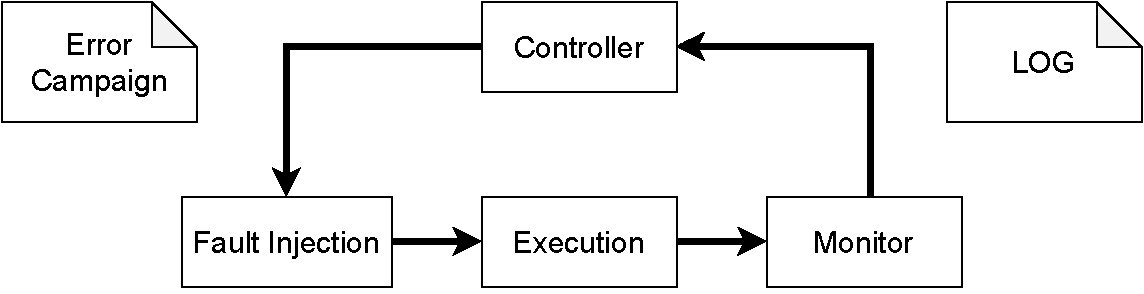
\includegraphics[width=0.95\linewidth]{images/chapter3/fi_env.pdf}
\caption{Basic scheme of a fault injection tool \cite{Ruano2021-wy}}
\label{fig:fi_example}
\end{figure}

In the general scheme, the following elements are present:

\begin{itemize}
    \item \textit{Controller}: it is the main application and the orchestrator of all the other components of the tools.
    \item \textit{Fault Injection}: it is the module responsible for injecting faults into the system, according to a specific error campaign.
    \item \textit{Execution}: the output of the fault injection is executed.
    \item \textit{Monitor}: the behavior of the system is monitored and logs are generated.
\end{itemize}

A widely accepted classification of the different injection strategies is summarized as follows:

\begin{description}
    \item[Hardware-Based fault injection] consists of the generation of physical errors into the integrated circuits. They can be divided into fault injections with contact and fault injections without contact. The one with contact consists in perturbating the integrated circuits via perturbation introduced at the pins (for example a rapid and minimal change of the power supply voltage) while in the case without contact there is an external source that produces physical phenomena such as heavy-ion radiations that induce faults in the integrated circuits.
    \item[Software-Based fault injection] consists of the generation of software errors. They can be artificially inserted into a software system, both at compile time or at run time. The ones at compile-time \cite{fithesisdrizz} are inserted into the source code of the software or at the assembly level after the compilation of the original source code itself. The ones at run-time are inserted through a trigger (for example a timeout or a software trap) that executes the fault injection module, altering the behavior of the software.
    \item[Simulation-Based fault injection] simulation-based fault injection is a technique that allows to simulate of the system and to inject faults into it. The faults are injected from within the simulation environment, and it can be done by modifying directly the high-level description of the design with a faulty model or by using built-in commands in the simulator that force error in the simulation of the design, not in the hardware description of the hardware itself. Example of simulation-based fault injection systems are SST \cite{4375147} and VERIFY \cite{614074}.
    \item[Emulation-Based fault injection] emulation-based fault injection is a technique consisting of a real implementation in an FPGA. For these platforms, the development board is connected to a PC that acts as a Controller by defining the fault injection campaign, controls the execution of the faulty design and monitors the behavior of the system under test.
\end{description}

The Fault Injection tool used is a kind of Emulation-Based fault injection \cite{fit}. Its goal is to create a faulty bitstream starting from the base one. Consequently, the faulty bitstream simulates a fault by forcing a random bit-flip, as a SEUs does. The tool offers the possibility to target a specific portion of the FPGA, in order to test the fault tolerance of a subpart of the design, instead of the whole one. This allows designers to execute a targeted fault campaign of the design under consideration. \bigskip

Thanks to tools like PyXEL \cite{8632000} it is possible to obtain a visual low-level representation of the bitstream. This allows an understanding of how and where the design's modules are mapped into the bitstream and consequently how each bit in the bitstream is connected to the design. Hence, by forcing some modules to stay in a specific portion of the FPGA, using some constraints as explained in chapter \ref{sec:bitstreamgen}, it is possible to understand the position of the modules in the bitstream. \bigskip

As a result, it is finally possible to have a targeted fault campaign. The Controller, part of the tool, can start producing $n$-faulty bitstreams, where $n$ is given as input by the user. Once all the faulty bitstreams are generated, the Controller starts the Execution part.\bigskip

As an important note, because of the bit-flips introduced into the bitstream, is necessary to remove any CRC checksum that may be present, that is checked during the upload in the FPGA, as explained in chapter \ref{sec:bitstreamgen}. To overcome this problem, Vivado must be instructed to generate a bitstream without CRC. It can be done with the following TCL commands:\bigskip

\begin{lstlisting}[style=tcl]
open_run impl_1
set_property BITSTREAM.GENERAL.CRC DISABLE [get_designs impl_1]
write_bitstream
\end{lstlisting}

The first execution only is related to the golden bitstream and the Monitor will capture the golden result, i.e. the correct and expected result. The result is intended as the \textit{stdout} output of a testbench firmware, over the UART. The firmware can implement, for example, a simple algorithm like matrix multiplication or bit count. Obviously, the more the algorithm is varied, in terms of used instructions and hardware, the more the chance to detect an injected fault, because of the higher probability to stimulate that fault. \bigskip

All the remaining Execution outputs are compared against the golden, thus each run is classified as correct or faulty. When the campaign ends, a summary is produced, as shown in the following example, extracted from a very small fault injection campaign:\bigskip

\begin{lstlisting}[style=preformatted]
Total injected bitflips = 17

    --- FUNCTIONAL ANALYSIS ---
Correct results     -> 14 [82.35%]
Faulty results(SDE) -> 0  [00.00%]
MicroBlaze halted   -> 3  [17.65%]
Total exceptions    -> 0  [00.00%]
\end{lstlisting}

\section{Integrated FPGA Debugger}
\label{sec:ila}

A powerful tool offered by Xilinx is the Integrated Logic Analyzer (ILA) IP. It is a logic analyzer core that can be used to monitor the internal signals of a design. The ILA core includes many advanced features of modern logic analyzers, including Boolean trigger equations, and edge transition triggers. Thus, it is possible to debug in real-time the internal behavior of the design directly by Vivado, without the need for external tools.\bigskip

To bebug a port, the ILA core must be instantiated, for example in a Block Design, and connected to the signals to debug. The configuration wizard allows to easily monitor an entire AXI bus or simple signals. 

\begin{figure}[H]
\centering
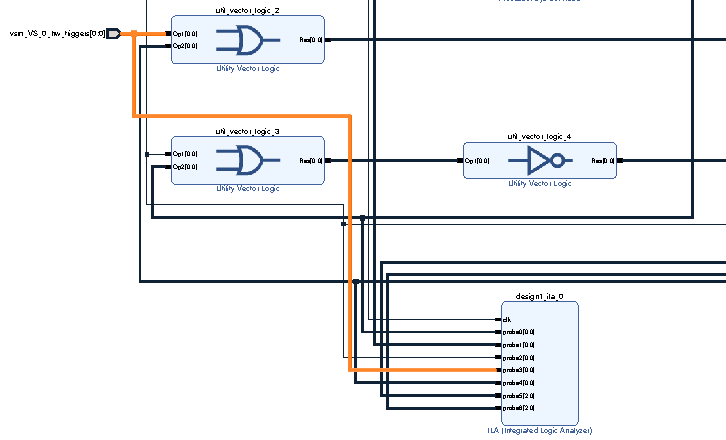
\includegraphics[width=0.65\linewidth]{images/chapter3/ila_inst_example_cropped_again_andagain.pdf}
\caption{Example of a ILA IP instantiation in a Block Design.}
\end{figure}

When the designer is satisfied with the number of signals to monitor, it is possible to continue with the normal Vivado Design Flow until the Implementation and Write Bitstream phases. The implementation requires a bit more effort due to the creation of the \textit{dbg_hub} core, which is the intermediary between the ILAs inserted into the design (where the signals to debug are connected) and the JTAG interface used to access and debug the design.\bigskip

To access the Debug functionalities, open Vivado's Hardware Manager and connect to the Hardware Server. If the FPGA is already configured, Vivado automatically opens the GUI to access and visualize all the signals and set various triggers. The GUI is similar to the one used to simulate the design:

\begin{figure}[H]
\centering
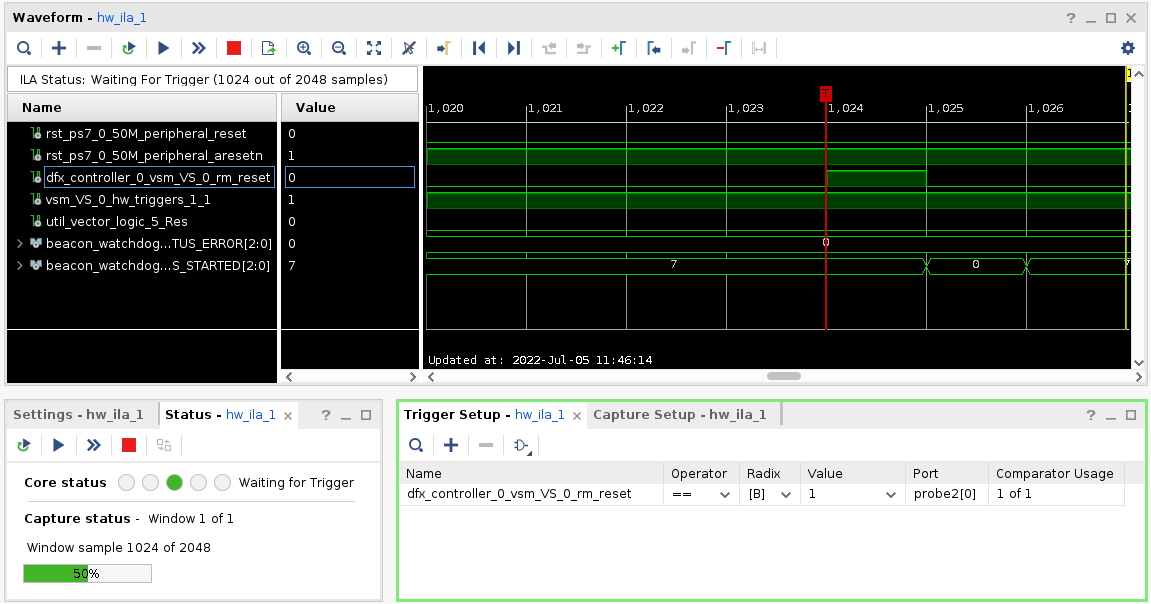
\includegraphics[width=0.80\linewidth]{images/chapter3/ila_example2.png}
\caption{ILA's debugging GUI in Vivado. The ILA is waiting for the trigger, and the trigger is set waiting to have a certain signal equal to 1.}
\end{figure}
